\immediate\write18{makeindex C-3.nlo -s nomencl.ist -o C-3.nls}
\documentclass[12pt,a4paper]{report}
\usepackage[utf8]{inputenc}
\usepackage{vietnam}
\usepackage[left=3cm, right=2.2cm, top=2.5cm, bottom=2.5cm]{geometry}
\usepackage{amsmath}
\usepackage{float}
\usepackage{amssymb} 
\usepackage{graphicx} 
\usepackage[hidelinks, unicode]{hyperref}
\usepackage[labelsep=period]{caption}
\usepackage[table]{xcolor}
\usepackage{titletoc}
\usepackage{etoc}
\usepackage{mathptmx}
\usepackage{sectsty}
\usepackage{multirow}
\usepackage{booktabs, tabularx}
\usepackage{courier}
\usepackage{subfig}
\usepackage{nomencl}
\usepackage{titlesec}
\usepackage{enumitem}
\usepackage{anyfontsize}
\usepackage[fontsize=13pt]{scrextend}
\newcommand{\code}[1]{\texttt{#1}}
\renewcommand{\baselinestretch}{1.5}
\renewcommand{\nomname}{Danh mục ký hiệu và viết tắt}


\makenomenclature
\makeatletter
\titlecontents{chapter}[3cm] % <-- seems to set some specific left margin
{\color{black}\bfseries\addvspace{3mm}}
{\makebox[0cm][r]{\MakeUppercase\@chapapp\hspace{.5em}\thecontentslabel\hspace{0.75cm}}}
{} %     ^^^ pretendously zero width box puts its contents in the left margin
{\hfill\makebox[-2cm]{\thecontentspage}}  % 3cm = twice 1.5cm
\chapternumberfont{\Large}
\chaptertitlefont{\Large}

\titleformat{\chapter}[hang] 
{\normalfont\fontsize{14}{15}\bfseries}{CHƯƠNG \thechapter.}{1em}{} 
\titlespacing*{\chapter}{0pt}{-7pt}{7pt}

\titleformat{\section}
{\normalfont\fontsize{13}{15}\bfseries}{\thesection.}{1em}{}
\titlespacing*{\section}{0pt}{-5pt}{-6pt}  

\titleformat{\subsection}
{\normalfont\fontsize{13}{15}\bfseries\itshape}{\thesubsection.}{1em}{}
\titlespacing*{\subsection}{0pt}{-20pt}{-6pt}

\titleformat{\subsubsection}
{\normalfont\fontsize{13}{15}\itshape}{\thesubsubsection.}{1em}{}
\titlespacing*{\subsubsection}{0pt}{-20pt}{-6pt}


\newcommand{\subsubsubsection}[1]{\paragraph{#1}\mbox{}\\}


\setlist[itemize]{itemsep=-0.3em, topsep=0pt}
\setlength\parindent{0pt}
\setlength{\parskip}{10pt}
\setcounter{secnumdepth}{4}
\setcounter{tocdepth}{4}
\geometry{letterpaper}

% \title{\textbf{ĐỒ ÁN CÔNG NGHỆ MỎ}}
% \author{Bùi Trọng Nghĩa\\Diệp Công Trứ}

\begin{document}
\pagenumbering{gobble}
% \thispagestyle{empty}
\clearpage

\pdfbookmark{\contentsname}{content}
% \maketitle

\tableofcontents
\addcontentsline{toc}{section}{MỤC LỤC}

\listoffigures
\addcontentsline{toc}{section}{DANH SÁCH HÌNH VẼ}

\listoftables
\addcontentsline{toc}{section}{DANH SÁCH BẢNG BIỂU}

\printnomenclature
\addcontentsline{toc}{section}{DANH MỤC KÝ HIỆU VÀ VIẾT TẮT}

\clearpage
\pagenumbering{arabic}
\newpage

\chapter{TRIỂN KHAI MÔ HÌNH}
\begin{center}
	\centering
	\textbf{A. XÂY DỰNG MÔ HÌNH DỰ BÁO THEO THỜI GIAN}
\end{center}
Ngôn ngữ lập trình được sử dụng trong luận án là Python và MATLAB.
\section{Tiền xử lý dữ liệu}
Tiền xử lý dự liệu là một bước cực kì quan trọng để có thể đưa ra đươc một kết quả tốt nhất, đặc biệt là đối với một bài toán thời gian. Tại bước này những dữ liệu ngoại lai, nhiễu, lặp, hoặc dữ liệu thiếu trong quá trình thu thập dữ liệu sẽ được xử lý nhằm cải thiện chất lượng dữ liệu và chất lượng kết quả.

Một vài kĩ thuật khác để tiền xử lý dữ liệu như tích hợp, biến đổi và thu giảm dữ liệu. Tuy nhiên, những kĩ thuật này yêu cầu có nguồn dữ liệu kích thước lớn, do đó phạm vi luận án sẽ không nhắc đến các kĩ thuật này.

Các dữ liệu ngoại lai, nhiễu, lặp, hoặc thiếu có thể được loại bỏ hay thay thế bằng giá trị trung bình hoặc trung vị của cả bộ dữ liệu. Source code của phần tiền xử lý này có thể được tìm thấy trên [link].

Đối với giếng X1, gồm 1710 điểm dữ liệu sẽ được xử lý còn 1020 điểm, trong đó loại bỏ 690 điểm có giá trị bằng 0, còn lại sẽ được thay thế bằng các giá trị trung bình. Dữ liệu trước và sau khi xử lý được thể hiện lần lượt trong hai Hình \ref{fig:before-process}, \ref{fig:after-process}.

Các giếng X2, X3, X4 sẽ được xử lý tương tự được thể hiện trong các hình ...

	\begin{figure}[h]
		\centering
		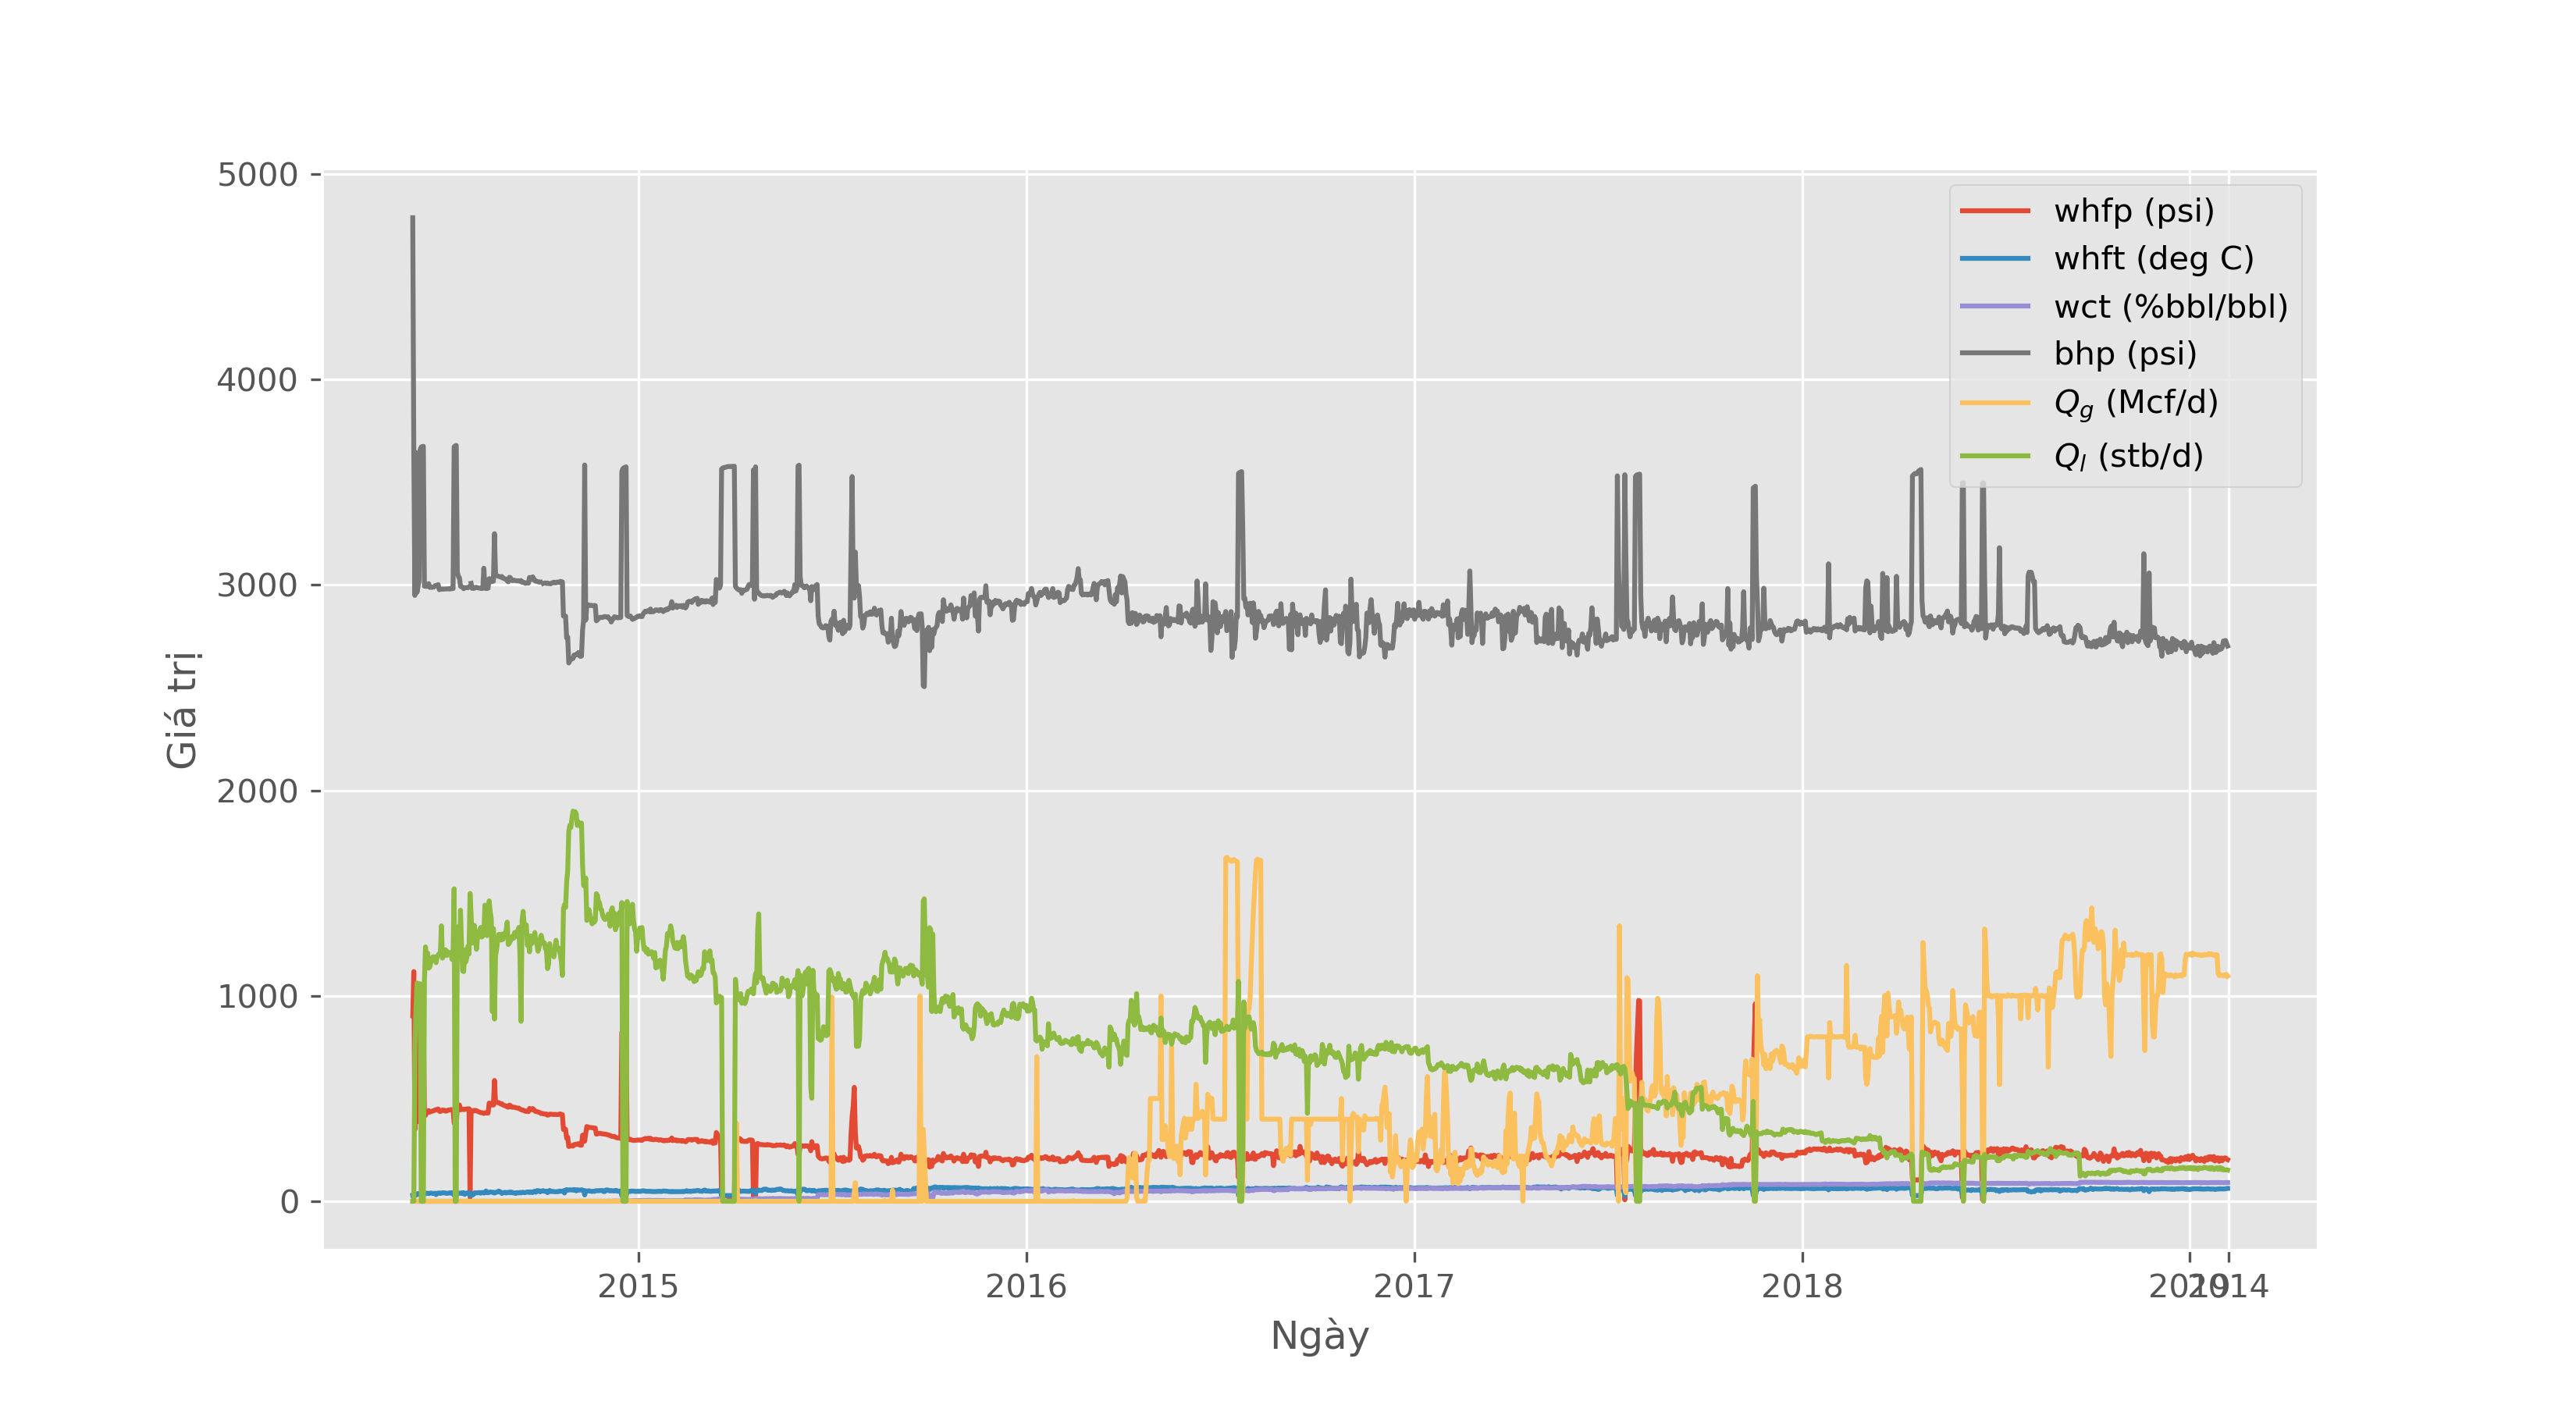
\includegraphics[scale=.6]{fig/before-process.png}
		\caption{Dữ liệu X1 trước khi xử lý}
		\label{fig:before-process}
	\end{figure}
	\begin{figure}[h]
		\centering
		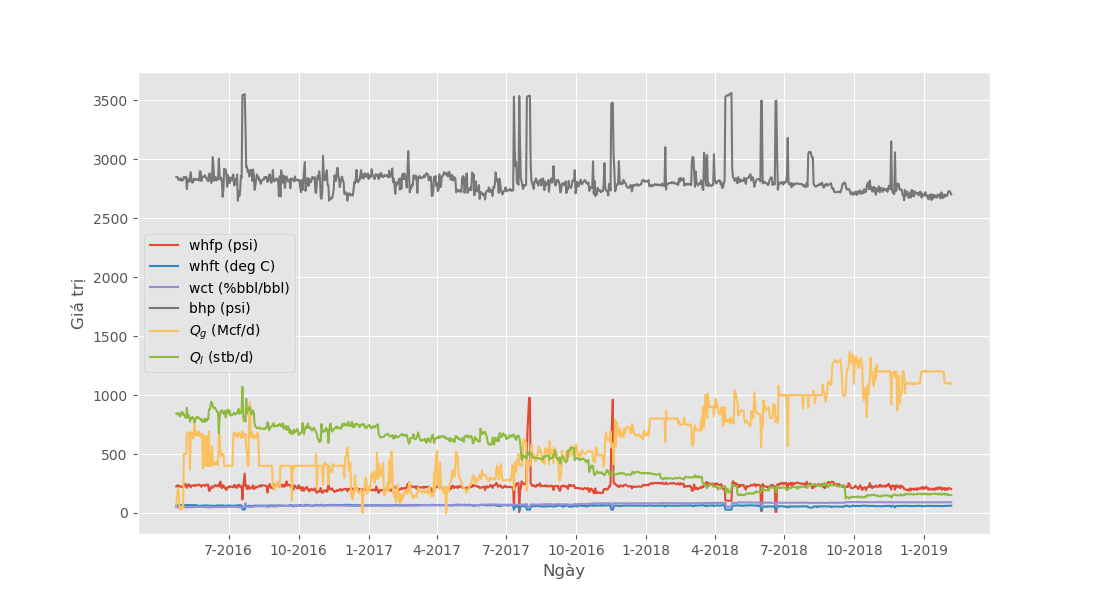
\includegraphics[scale=.6]{fig/after-process.png}
		\caption{Dữ liệu X1 sau khi xử lý}
		\label{fig:after-process}
	\end{figure}

\clearpage

\section{Xây dựng mô hình}
\subsection{Xây dựng cấu trúc}
Để đảm bảo dữ liệu đầu ra của mỗi mô hình phù hợp với dữ liệu đầu vào của mô hình giải thuật di truyền, quá trình xây dựng mô hình dự đoán sẽ xoay quanh các đặc tính dự đoán là nhiệt độ, áp suất đầu giếng, áp suất đáy giếng và hàm lượng nước.

Mỗi giếng sẽ được xây dựng bốn mô hình riêng biệt tương ứng với bốn đặc tính đã nêu ở trên. Tùy thuộc vào dữ liệu hiện có của mỗi giếng mà xác định cấu trúc mạng của mô hình. Với giếng X1 mô hình có thể được xây dựng với cấu trúc 3 phân lớp ẩn lần lượt có số lượng $unit$ là 32, 16, 16; phân lớp đầu vào sẽ có 8 $unit$ và một $unit$ của phân lớp đầu ra, cụ thể là mô hình dạng [8:32:16:16:1]. Hàm kích hoạt được sử dụng là $ReLU$, hàm tối ưu là $RMSProp$ cùng với phương pháp đánh giá là MSE. Tương tự, các giếng X2, X3, X4 sẽ có các cấu trúc lần lượng là ...\\

\subsection{Huấn luyện mạng}
Sau khi thiết lập cấu trúc cho từng mô hình, để có thể đưa mạng đã thiết lập vào huấn luyện cần bổ sung thêm các tham số huấn luyện khác bao gồm số vòng lặp ($epochs$), số điểm dữ liệu trong một vòng lặp (\textit{batch size}) và một vài thông số tự chọn khác như trộn dữ liệu ($shuffle$), tiến trình ($verbose$) ... Số $epochs$ sẽ được chọn cố định là 30 với tất cả các mô hình, số \textit{batch size} được lựa chọn ngẫu nhiên trong khoảng 8 đến 13, dữ liệu cũng sẽ được trộn để đảm bảo tính ngẫu nhiên.

Một số thuật toán tối ưu cổ điển yêu cầu khởi tạo tốc độ học (learning rate). Tuy nhiên, với tính chất tự thay đổi và cập nhật tốc độ học của các thuật toán hiện đại, điều này là không cần thiết.

Trước khi tiến hành huấn luyện, tập dữ liệu được chia thành hai phần, khoảng 80\% dữ liệu sẽ được sử dụng cho tập huấn luyện và 20\% cho tập kiểm thử. Kĩ thuật này giúp nâng cao tính khách quan trong quá trình dự báo đối với các điểm dữ liệu mới. Tiến trình huấn luyện được ghi lại thông qua biểu đồ sai số theo vòng lặp của hai tập huấn luyện và kiểm thử. Các biểu đồ này được thể hiện lần lượng trong ... tương ứng với 4 giếng X1, X2, X3, X4.\\

\subsection{Kết quả dự báo}
Sau khi quá trình huấn luyện hoàn thành, mạng sẽ được tiến hành kiểm tra hiệu suất dự báo trông qua tập kiểm thử, phương pháp đánh giá sử dụng là RMSE, MAPE, MASE. Các giá trị sai số này càng thấp chứng tỏ hiệu suất dự báo của mô hình càng cao. Giá trị dự báo được thể hiện trên đồ thị ... lần lượt cho từng thông số dự báo và cho từng giếng.

Cuối cùng, sau khi đánh giá hoàn tất, nếu mô hình đạt được yêu cầu về hiệu suất dự báo, mạng sẽ được đưa vào thực hiện dự báo cho thời gian kế tiếp (trong tương lai). Thời gian dự báo này có thể là ngày, tuần hoặc tháng tùy thuộc vào mục đích của người thực hiện đối với từng bài toán khác nhau.

Đối với bài toán lựa chọn lưu lượng bơm ép, tác giả thực hiện dự báo cho thời gian một ngày kế tiếp, cũng có nghĩa là sẽ tiến hành lựa chọn lưu lượng bơm cho cụm giếng ngày kế tiếp.

Ngày kết thúc ghi chép dữ liệu là 6/2/2019, do đó, mọi đặc tính cần thiết sẽ được dự báo cho ngày 7/2/2019. Dữ liệu dự báo được thể hiện trong Bảng ...

\begin{center}
	\centering
	\textbf{B. XÂY DỰNG MÔ HÌNH GIẢI THUẬT DI TRUYỀN}
\end{center}
\section{Triển khai thuật toán di truyền}
Mô hình giải thuật sẽ được triển khai cho 4 giếng X1, X2, X3, X4. Các thông số cần thiết cho quá trình tính toán bao gồm: ... Trong đó 4 thông số áp suất, nhiệt độ đầu giếng, áp suất đáy giếng và hàm lượng nước được lấy từ mô hình dự báo đặc tính giếng đã xây dựng ở Phần A.

Để quá trình tính toán được thuận tiện hơn, tác giả đã xây dựng một cơ sở dữ liệu dạng nhỏ. Cơ sở dữ liệu này bao hàm các thông số đã nêu ở trên, dữ liệu trong cơ sở có thể dễ dàng thêm hoặc bớt tùy theo số lượng giếng. Source code cho phần cơ sở dữ liệu có thể được tìm thấy tại [link].

Trong một mô hình giải thuật di truyền, ngoại trừ hàm lượng giá (fitness function) và thành phần nghiệm ($n_vars$) không thể thay đổi, các thông số xây dựng mô hình khác bao gồm: xác suất thực hiện phép lai ($p_c$), xác suất thực hiện phép đột biến ($p_m$), kích thước quần thể ($N$) được tác giả thực hiện lựa chọn qua nhiều lần tiến hành thực nghiệm.

Đầu tiên, khởi tạo quần thể $POP$ với kích thước $N = 100$. Trong đó, các nhiễm sắc thể được khởi tạo hoàn toàn ngẫu nhiên trong đoạn [0, 1], mỗi nhiễm sắc thể chứa 8 gen tương ứng với 8 thành phần nghiệm ($q_l, q_g$ của 4 giếng). Phép chọn được thực hiện theo phương thức cuộc đua (tournament selection) tức là sẽ lựa chọn nhiễm sắc thể có độ tương thích cao nhất theo hàm lượng giá.

Phép lai được thực hiện theo phương thức lai hóa đồng nhất nghĩa là các gen được chọn ra từ các cặp bố mẹ với xác suất bằng nhau. Xác suất thực hiện phép lai $p_c = 0.5$. Phép đột biến được thực hiện theo phương thức phân phối chuẩn tức gen được chọn sẽ được cộng thêm một giá trị ngẫu nhiên có phân phối chuẩn với biên dưới là 0 và biên trên là 1. Xác suất thực hiện phép đột biến $p_m = 0.1$.

Hàm lượng giá ở đây chính là hàm số [ref], được thực hiện cho 4 giếng. Như vậy, thông số của mô hình sẽ là:
	\begin{itemize}
		\item Kích thước quần thể $N = 100$
		\item Thành phần nghiệm $n_vars = 8$
		\item Xác suất thực hiện phép lai $p_c = 0.5$
		\item Xác suất thực hiện phép đột biến $p_m = 0.1$
		\item Hàm lượng giá là hàm số [ref]
	\end{itemize}



\end{document}